% !TeX program = latexmk
\documentclass{beamer}
\usepackage{amsmath}
\usetheme{metropolis}
\usepackage{eulervm}
\usepackage{tikz}
\usetikzlibrary{
    matrix, calc, chains, positioning, decorations.pathreplacing, arrows.meta, arrows, 
    shapes, tikzmark, bending, intersections, quotes, shapes.geometric
}

%\metroset{block=fill}

\title{Arithmétique à virgule flottante}
\author{Pablo de Oliveira (pablo.oliveira@uvsq.fr)}
\institute{M1 Calcul Haute Performance Simulation, Calcul Numérique}
\date{2024-2025}

\begin{document}
\maketitle

\begin{frame}{Sommaire}
    \tableofcontents
\end{frame}

\section{Standard IEEE-754}
\begin{frame}{Représentation des nombres flottants}
    IEEE-754 définit une représentation flottante standardisée.

    \[ f = s \times 2^e \times m \]

    \begin{center}
        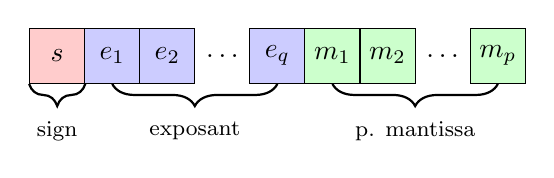
\begin{tikzpicture}
            \edef\sizetape{0.7cm}
            \tikzstyle{tmtape}=[draw,minimum size=\sizetape]
            \tikzstyle{tmhead}=[arrow box,draw,minimum size=.5cm,arrow box]

            \begin{scope}[start chain=1 going right,node distance=-0.15mm]
                \node (s) [on chain=1,tmtape, fill=red!20!white] {$s$};
                \node (es) [on chain=1,tmtape, fill=blue!20!white] {$e_1$};
                \node [on chain=1,tmtape, fill=blue!20!white] {$e_2$};
                \node [on chain=1,tmtape,draw=none] {$\ldots$};
                \node (ee) [on chain=1,tmtape, fill=blue!20!white] {$e_q$};
                \node (ms) [on chain=1,tmtape, fill=green!20!white] {$m_1$};
                \node [on chain=1,tmtape, fill=green!20!white] {$m_2$};
                \node [on chain=1,tmtape,draw=none] {$\ldots$};
                \node (me) [on chain=1,tmtape, fill=green!20!white] {$m_p$};
            \end{scope}

            \draw [thick,decorate,decoration={brace,amplitude=8pt,mirror}] (s.south west)
            -- (s.south east) node[midway,yshift=-.6cm] {\footnotesize sign};

            \draw [thick,decorate,decoration={brace,amplitude=8pt,mirror}] (es.south)
            -- (ee.south) node[midway,yshift=-.6cm] {\footnotesize exposant};

            \draw [thick,decorate,decoration={brace,amplitude=8pt,mirror}] (ms.south)
            -- (me.south) node[midway,yshift=-.6cm] {\footnotesize p. mantissa};
        \end{tikzpicture}
    \end{center}
    \begin{block}{Exemple}
        \begin{align*}
            (1.1010 \times 2^0)_2 =   & (1 \times 2^0 + 1 \times 2^{-1} + 0 \times 2^{-2} + 1 \times 2^{-3})_{10}                    \\
            =                         & (1 + 0.5 + 0.125)_{10} = 1.625_{10}                                                          \\                                                \\
            (1.1110 \times 2^{3})_2 = & (1 \times 2^{3} + 1 \times 2^{2} + 1 \times 2^{1} + 1 \times 2^0)_{10} = 15.0_{10}           \\
        \end{align*}
    \end{block}
\end{frame}

\begin{frame}[fragile]{Somme de deux flottants (example)}
    \begin{verbatim}
     1.1110               * 2^3
 +   1.1010               * 2^0
                <=>
     1.1110000            * 2^3
 +   0.0011010            * 2^3  (même exposant)
                                  ---> 3 bits
 -------------------------------
    10.0001010            * 2^3

     1.00001010           * 2^4  (renormalisation)
                                  <--- 1 bit
     16.625_10
    \end{verbatim}
\end{frame}

\begin{frame}{Standard IEEE-754}
    Formats classiques : binary32 (float), binary64 (double)

    Pour un double:
    \begin{itemize}
        \item 11 bits pour l'exposant, $e \in [-1022; 1023]$
        \item 52 bits de pseudo-mantisse (epsilon machine $\epsilon = 2^{-52}$)
    \end{itemize}

    Pseudo-mantisse car le premier bit est implicite
    \begin{itemize}
        \item 1 pour les normaux
        \item 0 pour les dénormaux
    \end{itemize}
\end{frame}

\begin{frame}{Encodage de l'exposant}
    L'exposant est codé avec biais, il faut soustraire 1023 ($ = 2^{q-1}-1$) à la valeur binaire $E=e_1\ldots e_q$
    \begin{itemize}
        \item pour l'exposant $2^1$, on stockera $E = 1024$ en binaire
        \item pour l'exposant le plus petit $2^{-1022}$, on stockera $E = 1$ en binaire
        \item pour l'exposant le plus grand $2^{1023}$, on stockera $E = 2046$ en binaire
    \end{itemize}

    \begin{block}{Valeur spéciales}
        \begin{itemize}
            \item $E = 2047$ représentent $+\infty, -\infty, NaN$ (en fonction de $s$ et $m$)
            \item $E = 0$ et $m = 0$ représentent +0 et -0
            \item $E = 0$ et $m \neq 0$ représente un dénormal
        \end{itemize}
    \end{block}
\end{frame}

\begin{frame}{Underflow et dénormaux}

    \begin{itemize}
        \item Le plus petit double normal (en valeur absolue): $ m = 1.0 \times 2^{-1022} $
        \item $\frac{m}{4}$ est non représentable car son exposant est trop petit; c'est un \emph{underflow}.
        \item Retourner la valeur $0$ à la place ? Pour ne pas
              perdre complètement la précision on utilise des dénormaux.
        \item On encode $ \frac{m}{4} = 0.01 \times 2^{-1022} $. Pour les dénormaux le bit implicite est remplacé par un zéro. Ici on perds deux bits de précision dans la mantisse.
    \end{itemize}
\end{frame}


\begin{frame}{Répartition sur la droite des réels}
    \begin{tikzpicture}
        \draw[-stealth] (0,0) -- (11,0) node[above]{$\mathbb{F}$};
        \edef\x{0}
        \foreach \e in {0.03125, 0.0625, 0.125, 0.25, 0.5, 1, 2, 4, 8}
            {
                \foreach \m in {1, 1.25, 1.5, 1.75}
                    {
                        \pgfmathparse{\e*\m}
                        \xdef\x{\pgfmathresult}
                        \draw (\x,-.1) -- (\x,0);
                    }
            }

        \draw (0,-.4) node[below]{$0$} -- (0,0);

        \draw (.25,.4) node[above]{$2^{-2}$} -- (.25,0);
        \draw (.5,-.4) node[below]{$2^{-1}$} -- (.5,0);
        \draw (1,.4) node[above]{$2^{0}$} -- (1,0);
        \draw (2,-.4) node[below]{$2^{1}$} -- (2,0);
        \draw (4,.4) node[above]{$2^{2}$} -- (4,0);
        \draw (8,-.4) node[below]{$2^{3}$} -- (8,0);

    \end{tikzpicture}

    Plus on se rapproche de zéro plus les flottants sont proches entre eux.
    Ici on a utilisé une précision $p=2$. Donc 4 valeurs possibles entre deux puissances de deux (1.00, 1.01, 1.10, 1.11).
\end{frame}


\begin{frame}{Arrondis}
    Si le résultat d'un calcul $x$ n'est pas représentable, il est arrondi.
    \begin{itemize}
        \item Mode au plus près: la valeur la plus proche est choisie (en cas d'équidistance, par défaut la mantisse paire est choisie).
        \item Vers $\pm\infty$ ou vers $0$: on arrondit vers $+\infty$, $-\infty$ ou $0$.
    \end{itemize}

    La norme IEEE-754 garantit l'arrondi correct pour + - $\times$ / $\sqrt{\,}$

    Lors d'un arrondi on commet une erreur maximale d' 1/2 ulp (unit in the last place).
    Soit pour un exposant $2^{0}$, on commet une erreur maximale de $\frac{\epsilon}{2} = u = 2^{-53}$.
\end{frame}

\section{Analyse d'Erreurs}
\begin{frame}{Modèle standard (Higham)}
    \[ fl(x \circ y ) = (x \circ y)(1+\delta) \qquad \text{ avec } |\delta| \le u = 2^{-53} \]
    \vfill{}
    Le terme $(1+\delta)$ capture l'erreur commise.
\end{frame}

\begin{frame}{Erreurs numériques: Représentation}
    \begin{itemize}
        \item Exemple: $0.1_{10} = 0.0001100110011\ldots_2$ a une mantisse infinie.
        \item La mantisse est tronquée en double précision.
    \end{itemize}
    \begin{block}{Bug du missile Patriot (1991)}
        \begin{itemize}
            \item Utilisation d'un registre de 24 bits pour multiplier 0.1 par l'horloge interne du système (pas de 0.1s).
            \item Après 100 heures, erreur d'approximation de 0.34s, soit 500m à la vitesse du missile Scud iraqien.
            \item Non interception du missile Scud, 34 soldats américains morts.
        \end{itemize}
    \end{block}
\end{frame}

\begin{frame}{Erreurs numériques: Absorption}
    \begin{itemize}
        \item Lors d'une addition ou soustraction, on renormalise le résultat.
        \item Les chiffres les plus à droite de la mantisse peuvent être perdus.
    \end{itemize}
    \hfill
    \center\includegraphics[height=2.5cm]{absorption.pdf}
\end{frame}

\begin{frame}{Erreurs numériques: Cancellation catastrophique}
    \begin{itemize}
        \item Lorsque l'on soustrait deux valeurs proches, une partie de la mantisse s'annule (en anglais on parle de \emph{cancellation})
              \begin{itemize}
                  \item $9633812.0 - 9633792.0 = 20.000000$
              \end{itemize}
              \vspace{.25cm}
              \includegraphics[width=.8\textwidth]{cancellation_example}
              \vspace{.25cm}
        \item On complète la mantisse avec des zéros.
        \item Si les deux opérandes contenaient des erreurs sur les derniers bits (erreur d'arrondi sur les opérations précédentes), c'est une \emph{cancellation catastrophique}.
        \item En effet, \textbf{l'erreur est promue en début de mantisse}.
    \end{itemize}
\end{frame}

\begin{frame}{Perte d'associativité}
    \begin{itemize}
        \item En raison des erreurs d'arrondi, absorption, cancellation, l'arithmétique IEEE-754 \textbf{n'est pas associative}.
              \[ a + (b + c) \ne (a + b) +c \]
        \item L'ordre des opérations est donc important.
    \end{itemize}
\end{frame}

\begin{frame}{Sources classiques d'erreur dans les codes de calcul}
    \begin{itemize}
        \item Sommations: produits scalaires, moyennes, réductions.
        \item Accumulation d'erreurs sur le temps: intégration méthodes explicites.
        \item Calcul de gradient sur des quantités proches.
        \item Non reproductibilité:
              \begin{itemize}
                  \item Parallélisme (change l'ordre des opérations)
                  \item Vectorisation et optimisations agressives
                  \item Branchements instables
              \end{itemize}
    \end{itemize}
\end{frame}
\begin{frame}{Quelques techniques pour atténuer les problèmes}
    \begin{itemize}
        \item Réécrire une expression pour éviter des cancellations catastrophiques ou absorptions.
              \[ \frac{\sqrt{x^2+1}-1}{x} = \frac{x}{\sqrt{x^2+1}+1} \qquad \text {cancellation pour } x \rightarrow 0 \]
        \item Remplacer une formule par une approximation qui se comporte correctement.
        \item Utiliser les bons facteurs d'échelle pour éviter les dépassements.
        \item Augmenter le précision.
        \item Utiliser des algorithmes compensés.
    \end{itemize}
\end{frame}

\begin{frame}{Analyse d'erreur en avant et en arrière}

    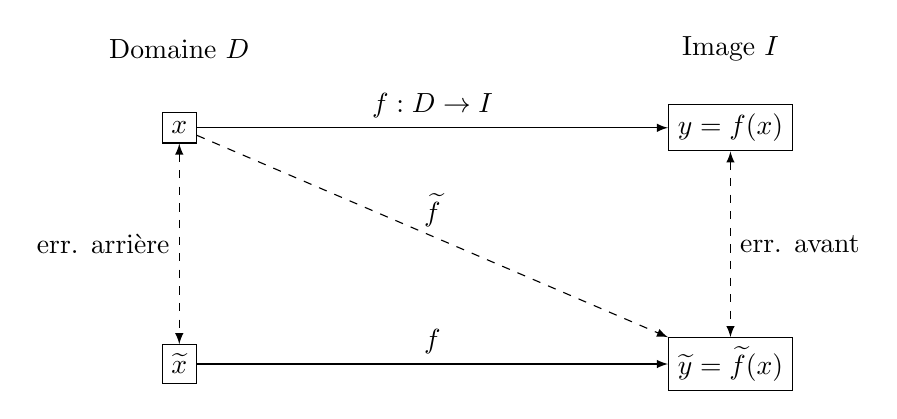
\begin{tikzpicture}
        \node at (0,0) {Domaine $D$};
        \node (x) [draw] at (0,-1) {$x$};

        \node at (7,0) {Image $I$};
        \node (fx) [draw] at (7,-1) {$y = f(x)$};



        \node (ftx) [draw] at (7,-4) {$\widetilde{y} = \widetilde{f}(x)$};


        \path (x)[draw,-latex] -- node[above] {$f: D \rightarrow I$} (fx) ;
        \path (x)[draw,-latex,dashed] -- node[above] {$\widetilde{f}$} (ftx) ;
        \path (fx)[draw,latex-latex,dashed] -- node[right] {err. avant} (ftx);

        \pause
        \node (xt) [draw] at (0,-4) {$\widetilde{x}$};

        \path (xt)[draw,-latex] -- node[above] {$f$} (ftx) ;
        \path (x)[draw,latex-latex,dashed] -- node[left] {err. arrière} (xt);
    \end{tikzpicture}

    \only<1>{
        Erreur avant $= \widetilde{y} - y$
    }
    \only<2>{
    \begin{itemize}
        \item Erreur arrière: on voit $\widetilde{y}$ comme l'image d'une entrée perturbée.
    \end{itemize}
    $$\widetilde{y} = f(\widetilde{x}) = f(x+\underbrace{\delta x}_{\textrm{err. arrière}})$$
    }

\end{frame}

\section{Étude de la somme}

\begin{frame}[fragile]{Exemple de la somme naïve}
    \begin{verbatim}
        sum = 0
        for i in range(n):
            sum += x[i]
    \end{verbatim}

    \[ f(\mathbf{x}) = S_n = \sum_{i=1}^n{x_i} \]
\end{frame}

\begin{frame}{Erreur en avant (Wilkinson, Higham)}
    \begin{align*}
        \widetilde{S}_k                                & = (\widetilde{S}_{k-1}+x_k)(1+\delta_k) \qquad |\delta_k| \le u,\, \delta_1 = 0,\, \widetilde{S}_0 = 0 \\
        \widetilde{S}_n                                & = \sum_{i=1}^n x_i \prod_{k=i}^{n}(1+\delta_k) \, \text { (récursivement) }                            \\
        \left| \prod_{k=i}^n{(1+\delta_k)} - 1 \right| & \le \sum_{k=i}^n{|\delta_k|} + O(u^2) \le (n-i+1)u + O(u^2)                                                  \\
        \left|\widetilde{S}_n - S_n \right|            & \le nu\sum_{i=1}^n{|x_i|} + O(u^2)                                                                     \\
    \end{align*}
\end{frame}

\begin{frame}{Erreur relative et Conditionnement de la somme}
    \begin{align*}
        \left|\widetilde{S}_n - S_n \right|               & \le nu\sum_{i=1}^n{|x_i|} + O(u^2)                                                                                           \\
        \frac{\left|\widetilde{S}_n - S_n \right|}{|S_n|} & \le   nu \underbrace{\left[\frac{\sum_{i=1}^n{|x_i|}}{ \left|\sum_{i=1}^n{x_i} \right|} \right]}_{Conditionnement}  + O(u^2)
    \end{align*}

    \begin{itemize}
        \item Si tous les termes sont de même signe, le conditionnement de la somme est 1.
              L'erreur numérique augmente linéairement avec le nombre d'opérations.
        \item En pratique, souvent les erreurs tendent à se compenser et l'augmentation de l'erreur est en $O(\sqrt{n})$.
    \end{itemize}
\end{frame}

\tikzstyle{vertex}=[draw,fill=black!15,circle,minimum size=20pt,inner sep=0pt]

\begin{frame}{Pairwise summation}
    Plutôt que de sommer les termes en série, il est possible de les sommer en arbre.
    \begin{tikzpicture}[very thick,level/.style={sibling distance=60mm/####1}]
        \node [vertex] (r){$+$}
        child {
                node [vertex] (a) {$+$}
                child {
                        node [vertex] {$x_1$}
                    }
                child {
                        node [vertex] {$x_2$}
                    }
            }
        child {
                node [vertex] {$+$}
                child {
                        node [vertex] {$x_{n-1}$}
                    }
                child {
                        node [vertex] {$x_n$}
                    }
            };
        \node at (0,-3cm) {$\ldots$};
    \end{tikzpicture}

    \begin{itemize}
        \item Erreur majorée par $O(log(n))$ et en pratique $O(\sqrt{log(n)})$
        \item D'autres algorithmes encore plus précis (Somme de Kahan)
    \end{itemize}
\end{frame}

\section{Arithmétique stochastique}

\begin{frame}{Arithmétique Stochastique (Stott Parker)}
    Problème: il est souvent difficile de faire une analyse formelle d'erreur pour un algorithme compliqué. Méthode empirique de mesure d'erreur ?

    \[ fl(x \circ y ) = (x \circ y)(1+\delta) \]

    \begin{itemize}
        \item On remplace $\delta$ par une variable aléatoire.

        \item On simule la distribution des erreurs arithmétiques d'un programme à
              l'aide de plusieurs tirages stochastiques.

        \item On choisit $\delta$ comme un bruit uniforme de magnitude $u$.
    \end{itemize}
\end{frame}


\begin{frame}{Arithmétique Stochastique (Stott Parker)}

    \begin{figure}
        \centering
        \includegraphics[width=.5\linewidth]{kahan.pdf}
        \caption{Erreur relative ($\frac{\sigma}{\mu}$). L'erreur pour la version naïve évolue en $O(\sqrt{n})$; la méthode compensée de Kahan est résistante au bruit numérique. Résultats obtenus avec le logiciel \url{https://github.com/verificarlo/verificarlo}}
    \end{figure}
\end{frame}

\begin{frame}{Références}
    \begin{itemize}
        \item GAO report -- Patriot Missile Defense, \url{https://www-users.cse.umn.edu/~arnold/disasters/GAO-IMTEC-92-96.pdf}
        \item The accuracy of floating-point summations, Nicholas Higham, 1993.
    \end{itemize}
\end{frame}


\end{document}
